% \textbf{how do we determine the overall membership}
% relevant info of the membership is in M12 table 1
% cannot determine the membership of two galaxies 
% spatial cut is defined in M12 p.9 first paragraph 

% paragraphs needs to be reorganized 
We adopt the identification of galaxy membership of El Gordo given by
\citepalias{M12} with a total count of 89 galaxies.
%The overall membership of the galaxies
%of El Gordo was first determined using a shifting gapper method
%\citep{Fadda96} after applying a rest frame cut of
%4000~\kilo\meter~\second$^{-1}$ \citep{Sifon13}. This method gives a
To further distinguish member galaxies of each subcluster, we adopt a
redshift cut of $z < 0.886$, and a spatial cut approximately perpendicular
to the 2D merger axis from \citetalias{M12} to determine that
there are 51 members in the NW subclusters and 35 members in the SE subclusters (See Figure
\ref{fig:membership}). 
The spatial cut indicated by the green line was done after
mapping the world coordinates to pixel coordinates to avoid anamorphic distortion. 

%Compare and contrast the amount of bootstrapping and the reported
%redshifts and velocity dispersion.
After identifying members of each subcluster, we performed 10, 000 bootstrap realizations to estimate the biweight
locations of the redshifts of the respective members in order to obtain the
samples of the PDFs of the redshifts of each subcluster. 
The spectroscopic redshift of the subclusters were
determined to be 
%$z_{total} = \pm $ 
$z_{\mathrm{NW}} = 0.86842 \pm 0.0011$ and 
$z_{\mathrm{SE}} = 0.87131 \pm 0.0012$, where the quoted numbers represent the
biweight location and 1$\sigma$ biased corrected confidence level
respectively \citep{Beers90}.  
%These biweight location estimators are less susceptible to outliers than
%the mean and standard deviations. 
Both the estimated redshifts of the subclusters and the uncertainties are
consistent with estimates given by \citealt{Sifon13}, and the fact that the
member galaxies of El
Gordo shows large velocity dispersion and has the largest velocity
dispersion among all the ACT galaxy clusters as reported by
\citetalias{M12}. These redshifts of the subclusters correspond to a
radial velocity difference in the frame of the NW subcluster
to be $476 \pm 242 $ km/s. We estimate the radial velocity differences of the
subclusters by first calculating the velocity of each subcluster with
respective to us, using  
\begin{equation}
	v_i = \left[ \frac{(1+z_i)^2 - 1 }{(1+z_i)^2 + 1 }\right]c
\end{equation}
where $c$ is the speed of light. And then the radial velocity was calculated
by: 
\begin{equation}
	\Delta v_{rad}(t_{obs}) = \frac{|v_2 - v_1|}{1-\frac{v_1 v_2}{c^2}}
\end{equation}
This result is lower than the the quoted radial velocity differences of
$586$
km/s reported by \citetalias{M12} from the approximation of $\Delta v_{rad}
= c(z_1 - z_2) / (1 + z_1)$ in the frame of the NW subcluster. 


\begin{figure}
	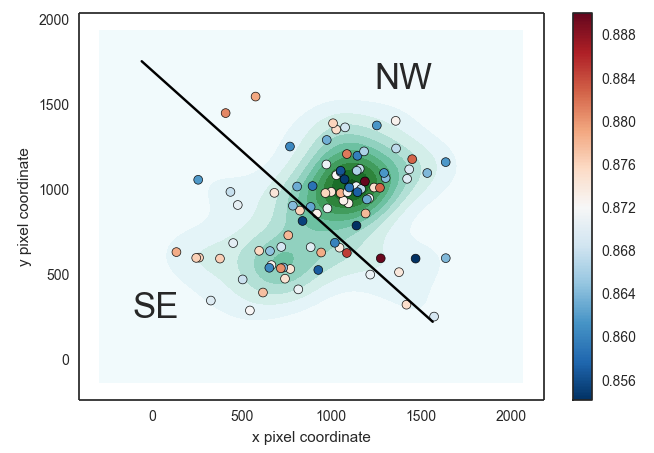
\includegraphics[width = \linewidth]{confirmed_member_divide.png}
	\caption{\label{fig:membership} The division of
the member galaxies among the two subclusters of El Gordo by a spatial cut
(green line). The color bar shows the color mapping of the spectroscopic
redshift of the member galaxies, with the redder end indicating higher
redshift.} 
\end{figure}

%We confirm the existence of the subclusters of El Gordo from the 2D spatial
%location of the galaxies, with the more massive cluster lying in the
%northwest (NW) and the less massive subcluster lying in the southeast(SE)  (REF - also have to reference the other literature
%for confirmation in the other wavelengths)
%
%Specifically, the membership of the NW and SE subclusters are
%determined based on a combination of the redshift and the spatial location. 
